\section{Sequential Modeling}

	\begin{figure}[htbp]
		\centering
		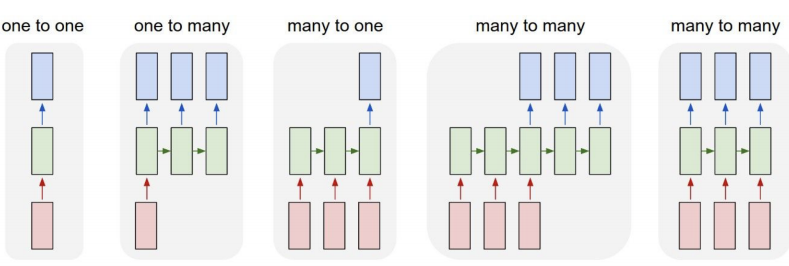
\includegraphics[scale=0.65]{figures/rnn-seqdata.png}
		\caption{各种输入输出方式}
	\end{figure}

	我们之前的网络,都是one-to-one,一个输入,一个输出.
	
	one-to-many:例如看图说话, Image Captioning, image$\rightarrow$sequence of words
	
	many-to-one:例如动作预测.
	
	many-to-many:例如video captioning, 或者 video captioning, 可以看作是沿着时间维度的 action segmentation.

	此外还有offline和online的处理.前者全部看完,后者边看边输出.
	
	\subsection{Recurrent Neural Network (RNN)}
	
	还有 recursive NN, 但是不常用

	Key idea: RNNs have an "internal state" that is updated as a sequence is processed

	这个输出就是 $h$, hidden state

	\begin{figure}[htbp]
		\centering
		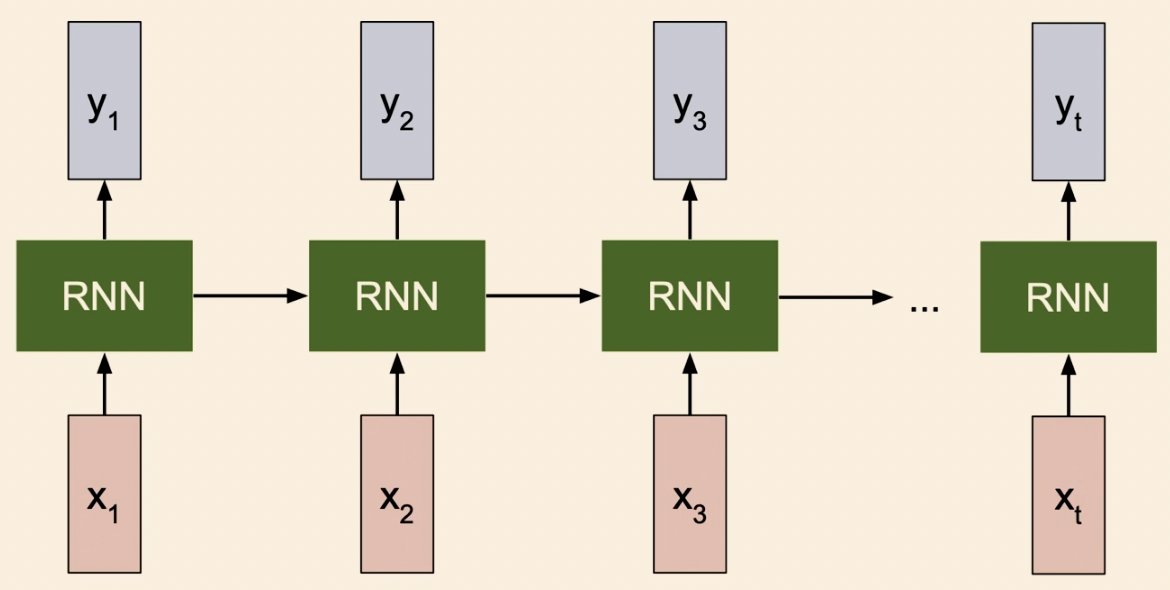
\includegraphics[scale=0.3]{figures/rnn.png}
		\caption{RNN: 典型的 many-to-many}
	\end{figure}

	值得注意的是, RNN 的架构很灵活, 可以容易改变输出输出从而变成 many-to-one, one-to-many 等等

	\begin{equation}
		\begin{cases}
			h_t = f_W\xk{h_{t-1}, x_t}
			\\
			y_t = f_{W_{hy}}\xk{h_t}
		\end{cases}
	\end{equation}

	输出的 $y_t$ 作为一个 decoder, 在需要输出结果的时候输出,否则不输出

	最开始的 $h_0$ 一般是全零的, 也可以是随机的,只要一样就行

	\subsection{Vanilla RNN}

	最初始的RNN

	P.S. 叫做 vanilla 是因为它是最原始的

	\begin{equation}
		\begin{cases}
			h_t = \tanh\xk{W_{hh}h_{t-1} + W_{xh}x_t}
			\\
			y_t = W_{hy}^*h_t
		\end{cases}
	\end{equation}
	
	计算图,各个方向流向W:
	
	\begin{figure}[htbp]
		\centering
		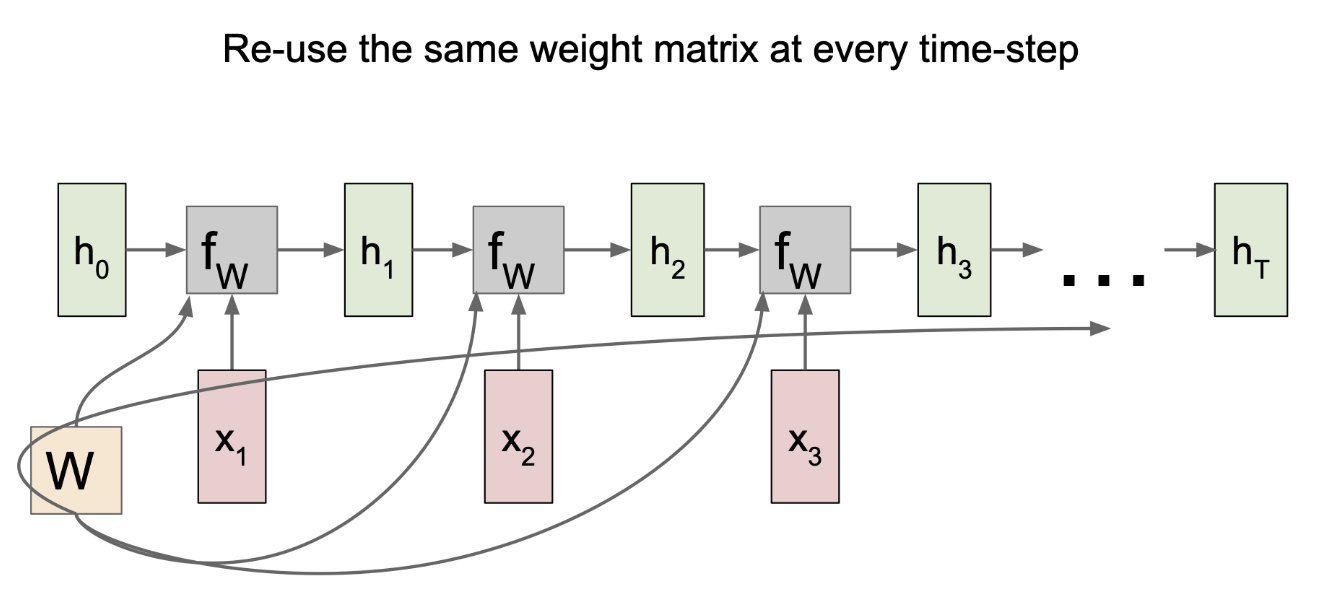
\includegraphics[scale=0.35]{figures/vanilla_rnn.png}
		\caption{Vanilla RNN Computational Graph}
	\end{figure}
	
	\subsubsection{Characer-Level Language Model}

	\begin{figure}[htbp]
		\centering
		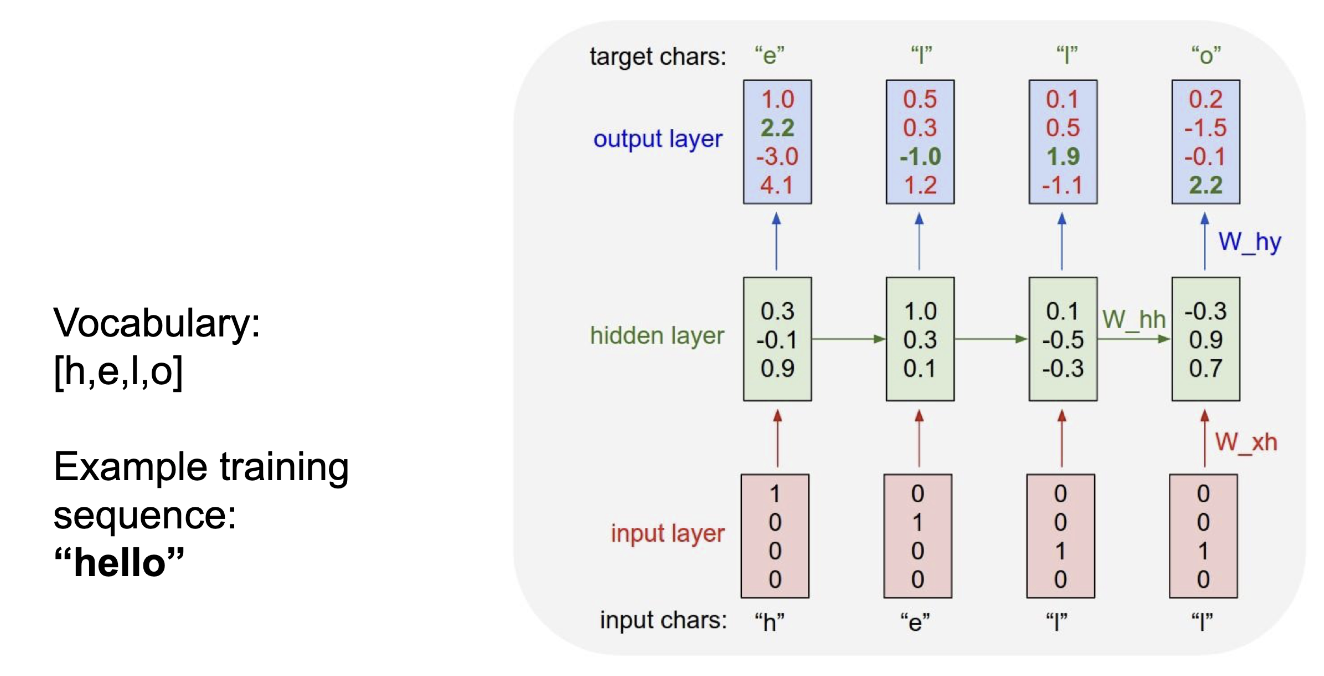
\includegraphics[scale=0.3]{figures/word_model.png}
		\caption{Characer-Level Language Model}
	\end{figure}

	先考虑简单的模型, character-level language model, 有限集合的字符, 
	比如英文26个字母, 逗号, 句号等等

	BP时,不同位置的W被loss调用了不同次.这个操作开销极大.

	\begin{figure}[htbp]
		\centering
		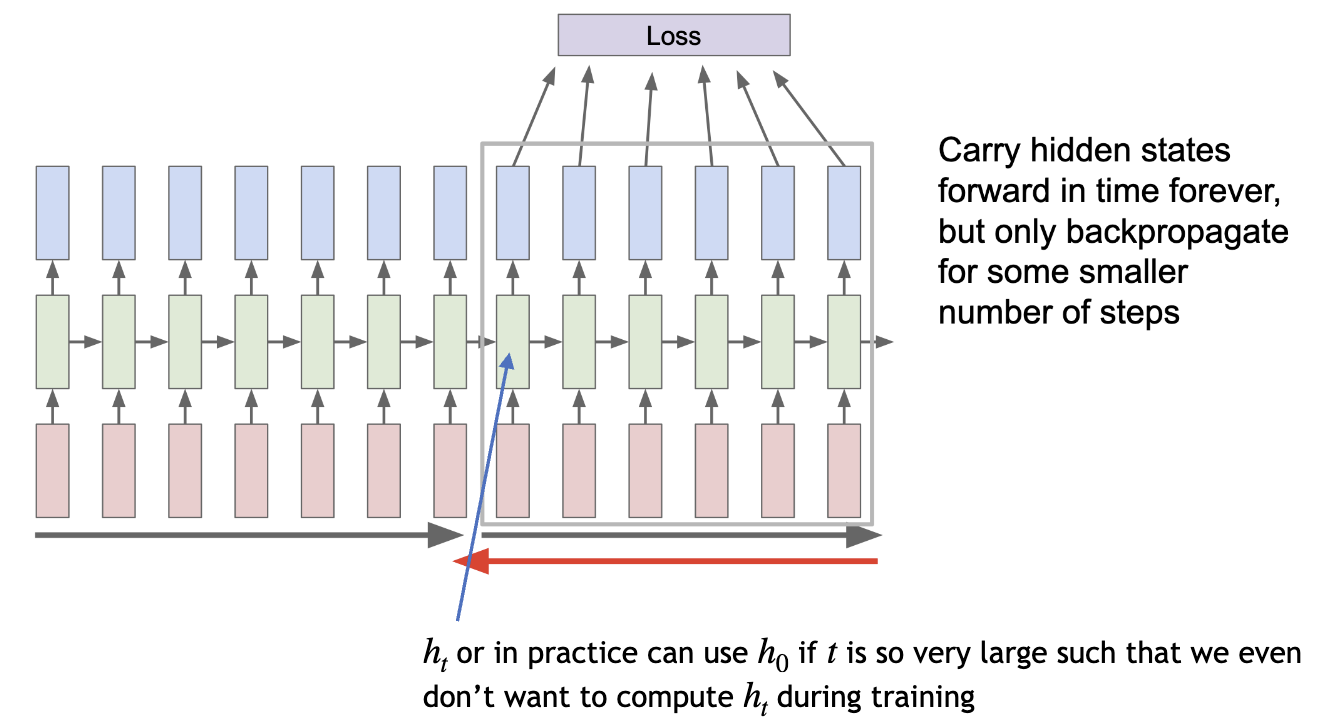
\includegraphics[scale=0.3]{figures/truncate_bp.png}
		\caption{Truncated BP}
	\end{figure}
	
	解决方法:truncated BP截断回传.比如FP时是从0到t,BP只算从t到t-6.

	这个window length是sequence length

	\subsubsection{Why share weight?} 
	Just like the CNN, we want the word features to be equalvariant. 
	Same sentence, different position in the article, should have the same feature.

	\subsubsection{Different Sampling Strategies}
	\begin{itemize}
		\item Greedy sampling: always takes the highest prob.
		
		Issue: deterministic, can only generate one sequence given
		the initial token and hidden states.
		\item Weighted sampling: sample the next token according to the
		predicted probability distribution
		
		Advantage: can generate diverse sequences.
		
		Issue: can accidentally obtain wrong token and screw up the
		generation.
		\item Exhaustive Search
		\[
		\begin{aligned}P(y|x)&=P(y_1|x)P(y_2|y_1,x)P(y_3|y_1,y_2,x)\ldots,P(y_T|y_1,\ldots,y_{T-1},x)\\&=\prod_{t=1}^TP(y_t|y_1,\ldots,y_{t-1},x)\end{aligned}
		\]
		\item Beam Search: top K most likely, next time, select K from KV results.
	\end{itemize}
	
	实际上将h和x结合的时候,常常先将x进行embedding, W [h,x]->W [h, g (x)].
	比如,hidden layer可能之后512维,但是输入如果是词向量,那么可能有几万维,
	非常不均衡.因此将embedding到合适的维度.此外,word embedding已经有现成的处理.
	
	RNN在长程记忆里会出现问题.delta t一般被称为sequence length.如果过短则相关性不强,过长则cost过多.
	
	\subsection{RNN tradeoff}
	\begin{itemize}
		\item RNN Advantages:
		\begin {itemize}
			\item Can process any length input
			\item Computation for step t can (in theory) use information from many steps back
			\item Model size doesn't increase for longer input
			\item Same weights applied on every timestep, so there is symmetry in how inputs are processed.
		\end{itemize}
		\item RNN Disadvantages:
		\begin{itemize}
			\item Recurrent computation is slow
			\item In practice, difficult to access information from many steps back
		\end{itemize}
	\end{itemize}

	\subsection{Multilayer RNNs}
	\begin{figure}[htbp]
		\centering
		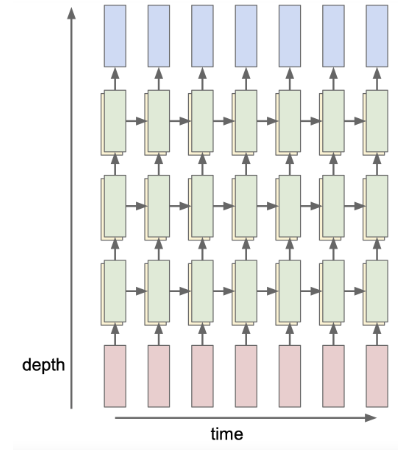
\includegraphics[scale=0.35]{figures/multilayer_rnn.png}
		\caption{Multilayer RNN}
	\end{figure}

	增强RNN非线性的能力
	
	\subsection{Vanilla RNN Gradient Flow}

	\begin{figure}[H]
		\centering
		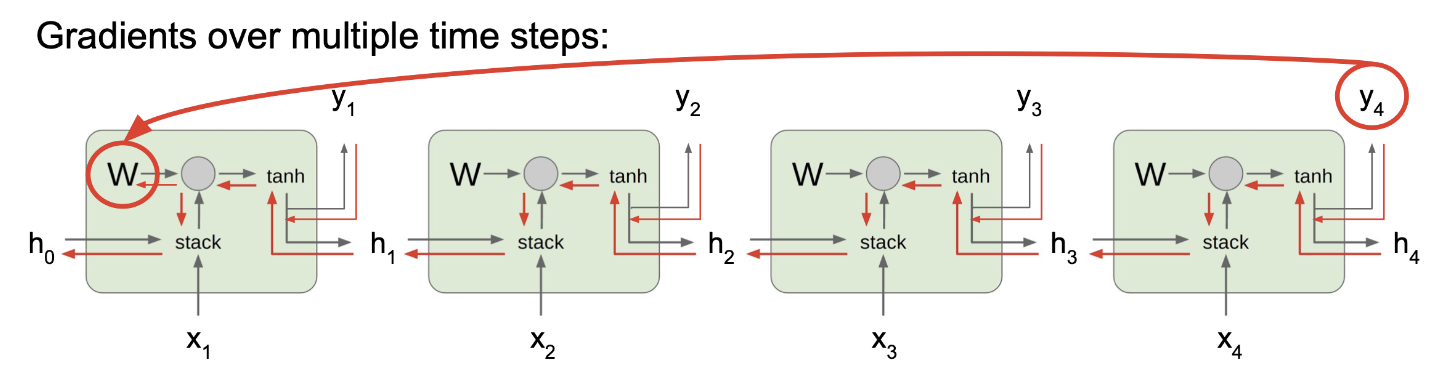
\includegraphics[scale=0.3]{figures/RNN_grad_van.png}
		\caption{Vanilla RNN Gradient Flow}
	\end{figure}

	\[
	\begin{aligned}
		h_{t}& =\tanh(W_{hh}h_{t-1}+W_{xh}x_{t})  \\
		&=\tanh\left(\begin{pmatrix}W_{hh}&W_{hx}\end{pmatrix}\begin{pmatrix}h_{t-1}\\x_t\end{pmatrix}\right) \\
		&=\tanh\left(W\begin{pmatrix}h_{t-1}\\x_t\end{pmatrix}\right)
		\end{aligned}	
	\]
	
	tanh的梯度恒小于1,梯度消失:

	\[
		\frac{\partial h_t}{\partial h_{t-1}}=tanh^{\prime}(W_{hh}h_{t-1}+W_{xh}x_t)W_{hh}	
	\]

	\[
		\frac{\partial L_T}{\partial W}=\frac{\partial L_T}{\partial h_T}\frac{\partial h_t}{\partial h_{t-1}}\ldots\frac{\partial h_1}{\partial W}=\frac{\partial L_T}{\partial h_T}(\prod_{t=2}^T\frac{\partial h_t}{\partial h_{t-1}})\frac{\partial h_1}{\partial W}	
	\]

	Gradient signal from far away is lost because it's much smaller than 
	gradient signal from close-by.

	Model weights are updated only with respect to near effects, not 
	long-term effects.
	
	\textbf{gradient clipping}对于exploding grad有一定作用, 但是解决不了 vanishing gradient 的问题.必须Change RNN architecture
	
	\subsection{LSTM}

	\[
	\begin{aligned}
		\begin{pmatrix}i\\f\\o\\g\end{pmatrix}& =\begin{pmatrix}\sigma\\\sigma\\\sigma\\\tanh\end{pmatrix}W\begin{pmatrix}h_{t-1}\\x_t\end{pmatrix}  \\
		&c_{t} =f\odot c_{t-1}+i\odot g  \\
		&h_{t} =o\odot\tanh(c_t) 
	\end{aligned}
	\]

	i: Input gate, whether to write to cell
	f: Foraet gate. Whether to erase cell
	o: Output gate, How much to reveal cell
	g: Gate gate (?), How much to write to cell
	
	cell state是long-term memory.我们知道对于普通的tanh,往01之间映射,那么$h_t$和很早之前的$h_i$之间的联系就比较微弱了.
	而LSTM中的c则一直把信息保留(f也是经过sigmoid激活的,在01之间,可以选择记住或者遗忘),最后h将c进行处理.
	
	核心结构:old info和new info的加和.若f=1,则就是skiplink.换言之c之间有梯度的旁路.

	\begin{figure}[htbp]
		\centering
		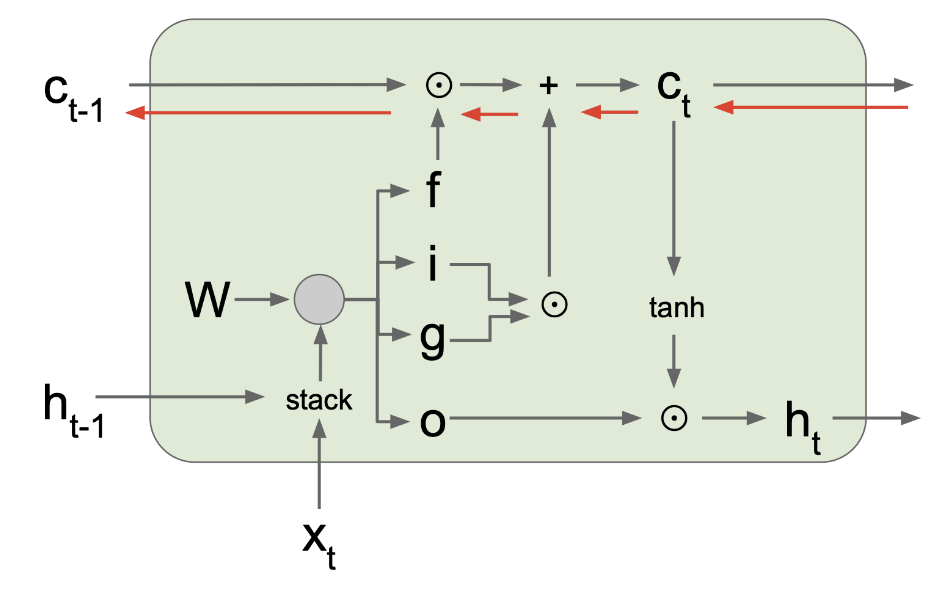
\includegraphics[scale=0.35]{figures/lstm_grad_flow.png}
		\caption{LSTM Gradient Flow}
	\end{figure}

	因为c是旁路,梯度可以直接流过来

	\subsubsection{Do LSTMs Solve the Vanishing Gradient Problem?}

	不能保证. 但是这种skip link的结构可以缓解这个问题.

	Long term dependencies 的问题得到了很好的解决

	\subsection{Gated Recurrent Unit (GRU)}

	\[
	\begin{aligned}
		&r_{t} =\sigma(W_{xr}x_t+W_{hr}h_{t-1}+b_r)  \\
		&z_{t} =\sigma(W_{xz}x_t+W_{hz}h_{t-1}+b_z)  \\
		&\tilde{h}_{t} =\tanh(W_{xh}x_t+W_{hh}(r_t\odot h_{t-1})+b_h)  \\
		&h_t =z_t\odot h_{t-1}+(1-z_t)\odot\tilde{h}_t 
	\end{aligned}	
	\]

	性能不输LSTM, 有的时候还更好

	了解即可

	\subsection{Summary}

	LSTM是一种RNN, 所有Sequencial Model都是RNN, 只是不是vanilla RNN